\documentclass[problem]{mcs}

\begin{pcomments}
  \pcomment{MQ_isomorphic_but_not_planar}
  \pcomment{from: S10.mq4}
\end{pcomments}

\pkeywords{
  simple_graphs
  isomorphism
  planar_graphs
  planar_embeddings
}

%%%%%%%%%%%%%%%%%%%%%%%%%%%%%%%%%%%%%%%%%%%%%%%%%%%%%%%%%%%%%%%%%%%%%
% Problem starts here
%%%%%%%%%%%%%%%%%%%%%%%%%%%%%%%%%%%%%%%%%%%%%%%%%%%%%%%%%%%%%%%%%%%%%

\begin{problem}
\bparts

\ppart
For the planar embeddings picture below, list all the discrete faces 
(simple cycles that define the region borders).

\begin{center}
  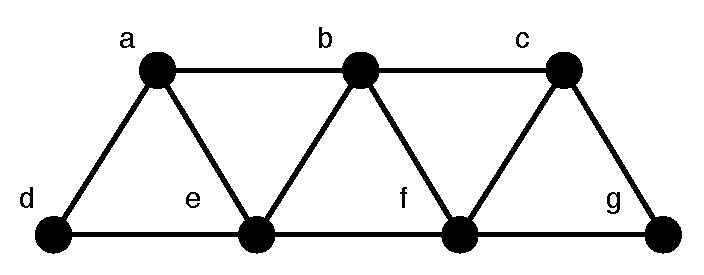
\includegraphics[height=1in]{figures/planar_graph.pdf}
\end{center}

\examspace[2in]

\begin{solution}
  adea, abea, befb, bcfb, cfgc, abcgfeda
\end{solution}

\ppart
Describe the discrete faces of a different planar embeddings for the 
graph in the previous part.

\examspace[4in]

\begin{solution}
  The graph below has the following faces:
  adea, abea, befb, bcgfb, cfgc, abcfeda
  
  \begin{center}
    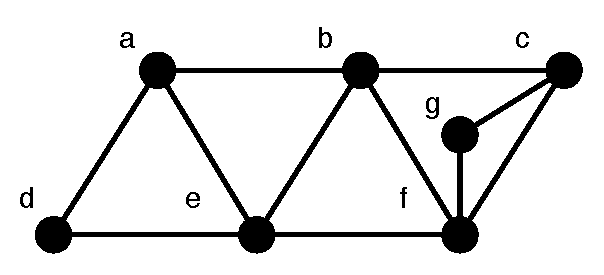
\includegraphics[height=1in]{figures/planar_graph_folded.pdf}
  \end{center}
  
\end{solution}

\eparts

\end{problem}

%%%%%%%%%%%%%%%%%%%%%%%%%%%%%%%%%%%%%%%%%%%%%%%%%%%%%%%%%%%%%%%%%%%%%
% Problem ends here
%%%%%%%%%%%%%%%%%%%%%%%%%%%%%%%%%%%%%%%%%%%%%%%%%%%%%%%%%%%%%%%%%%%%%

\endinput
